\section{Optimization Techniques on GPU}
\label{optimization}

In this section, we presents the optimization techniques on GPU to improve the algorithm efficiency.

\subsection{Eliminating Cyclic Paths and Atomic Operations}
\label{eliminate}
When the recursion-based coloring algorithm works on cyclic graphs, it is easy to fall into an infinite loop since 
the algorithm runs following the edge's direction. In order to solve this problem, we develop a method in Feluca to eliminate the cyclic paths in the directed graphs. In the method, Feluca checks all the vertices $v_j \in V_i$ (i.e., the set of neighbours of vertex $v_i$) before coloring $v_i$, and changes the edge $<v_i, v_j>$ to $<v_j, v_i>$, if $i>j$. For example, the edge $<v_4, v_1>$ in figure \ref{fig:color_a} is changed to $<v_1, v_4>$ in figure \ref{fig:color_b}. The change of edge direction does not affect the coloring plan. For example, these two coloring scheme in figure \ref{fig:color_a} and figure \ref{fig:color_b} are regarded as same.  

\begin{figure}[h]
\centering
\subfloat[Cyclical graph coloring]{%
\label{fig:color_a}
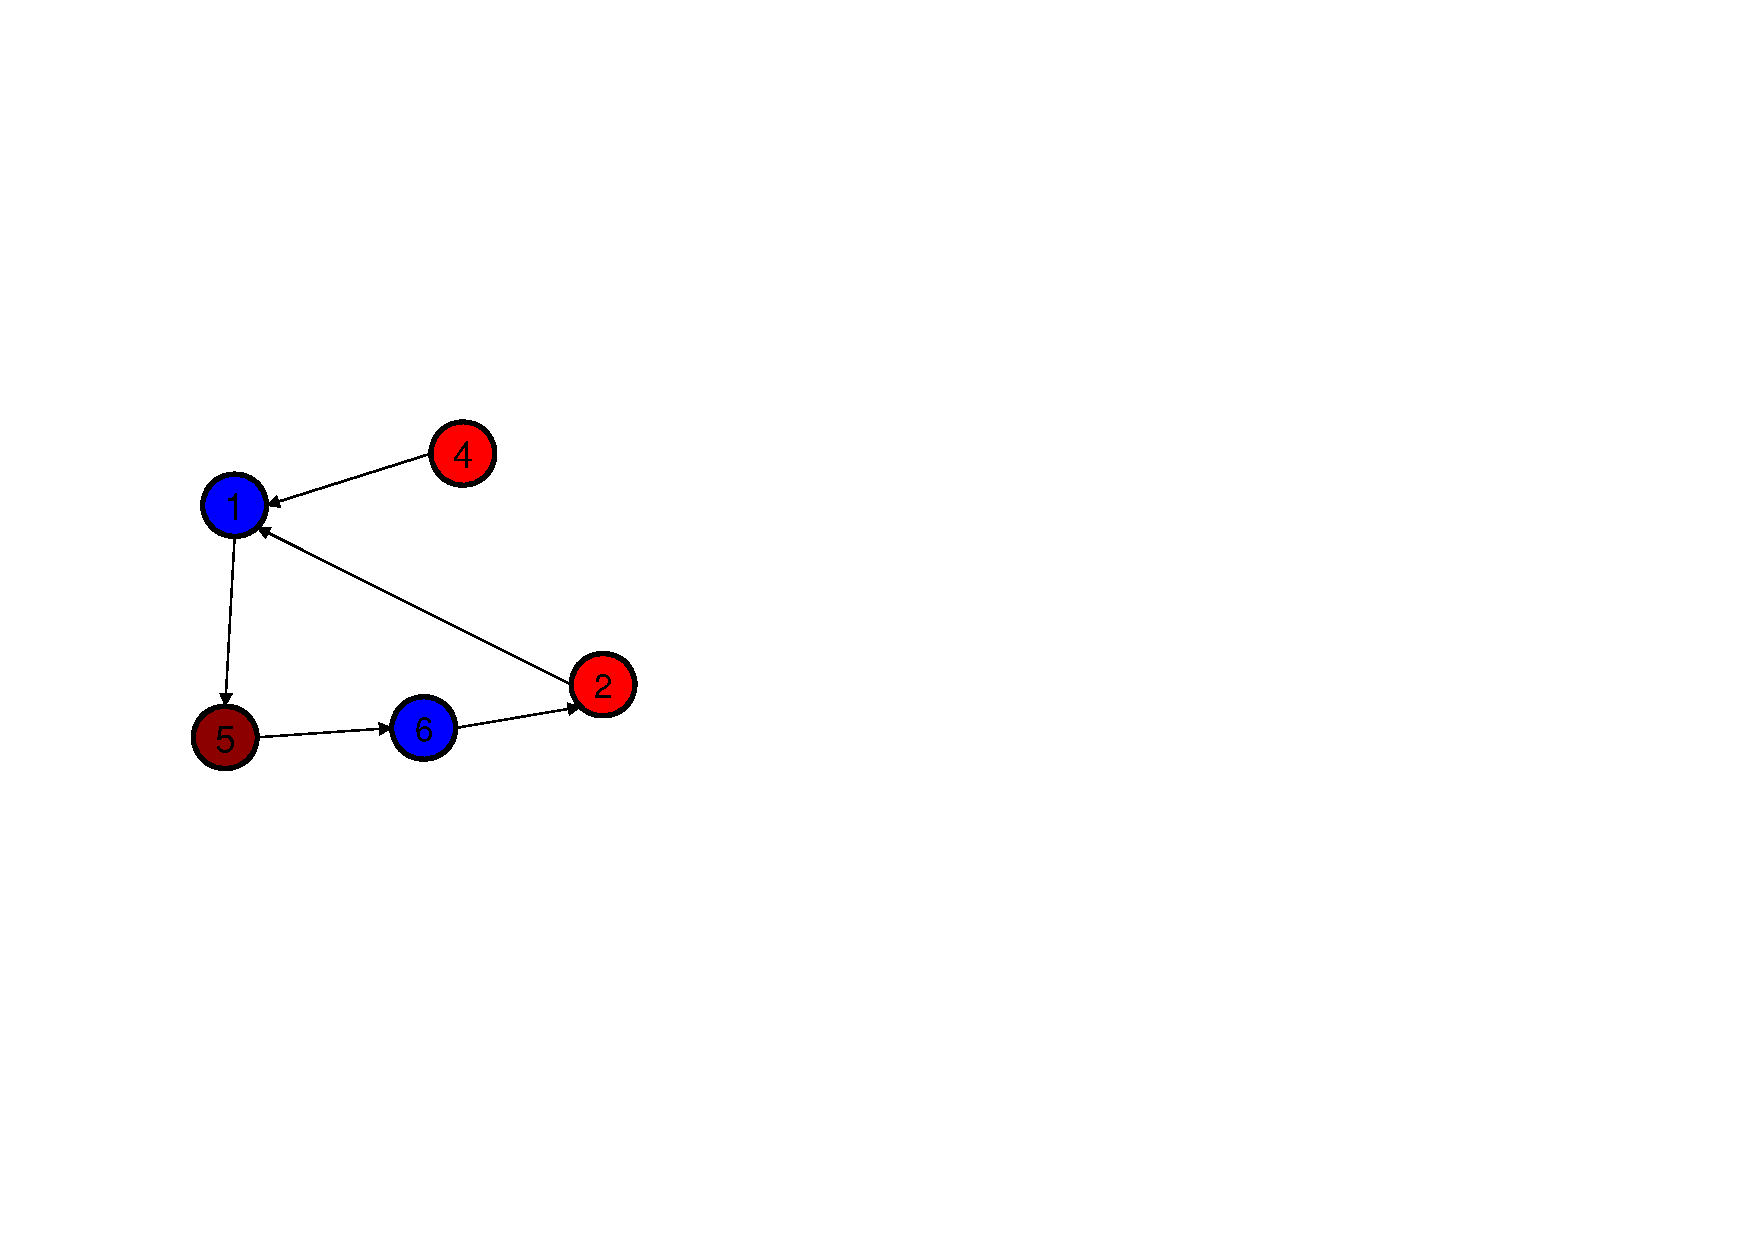
\includegraphics[scale=0.4]{figure/color_b.pdf}
}%
\hspace{0.4in}
\subfloat[Acyclic graph coloring]{
\label{fig:color_b}
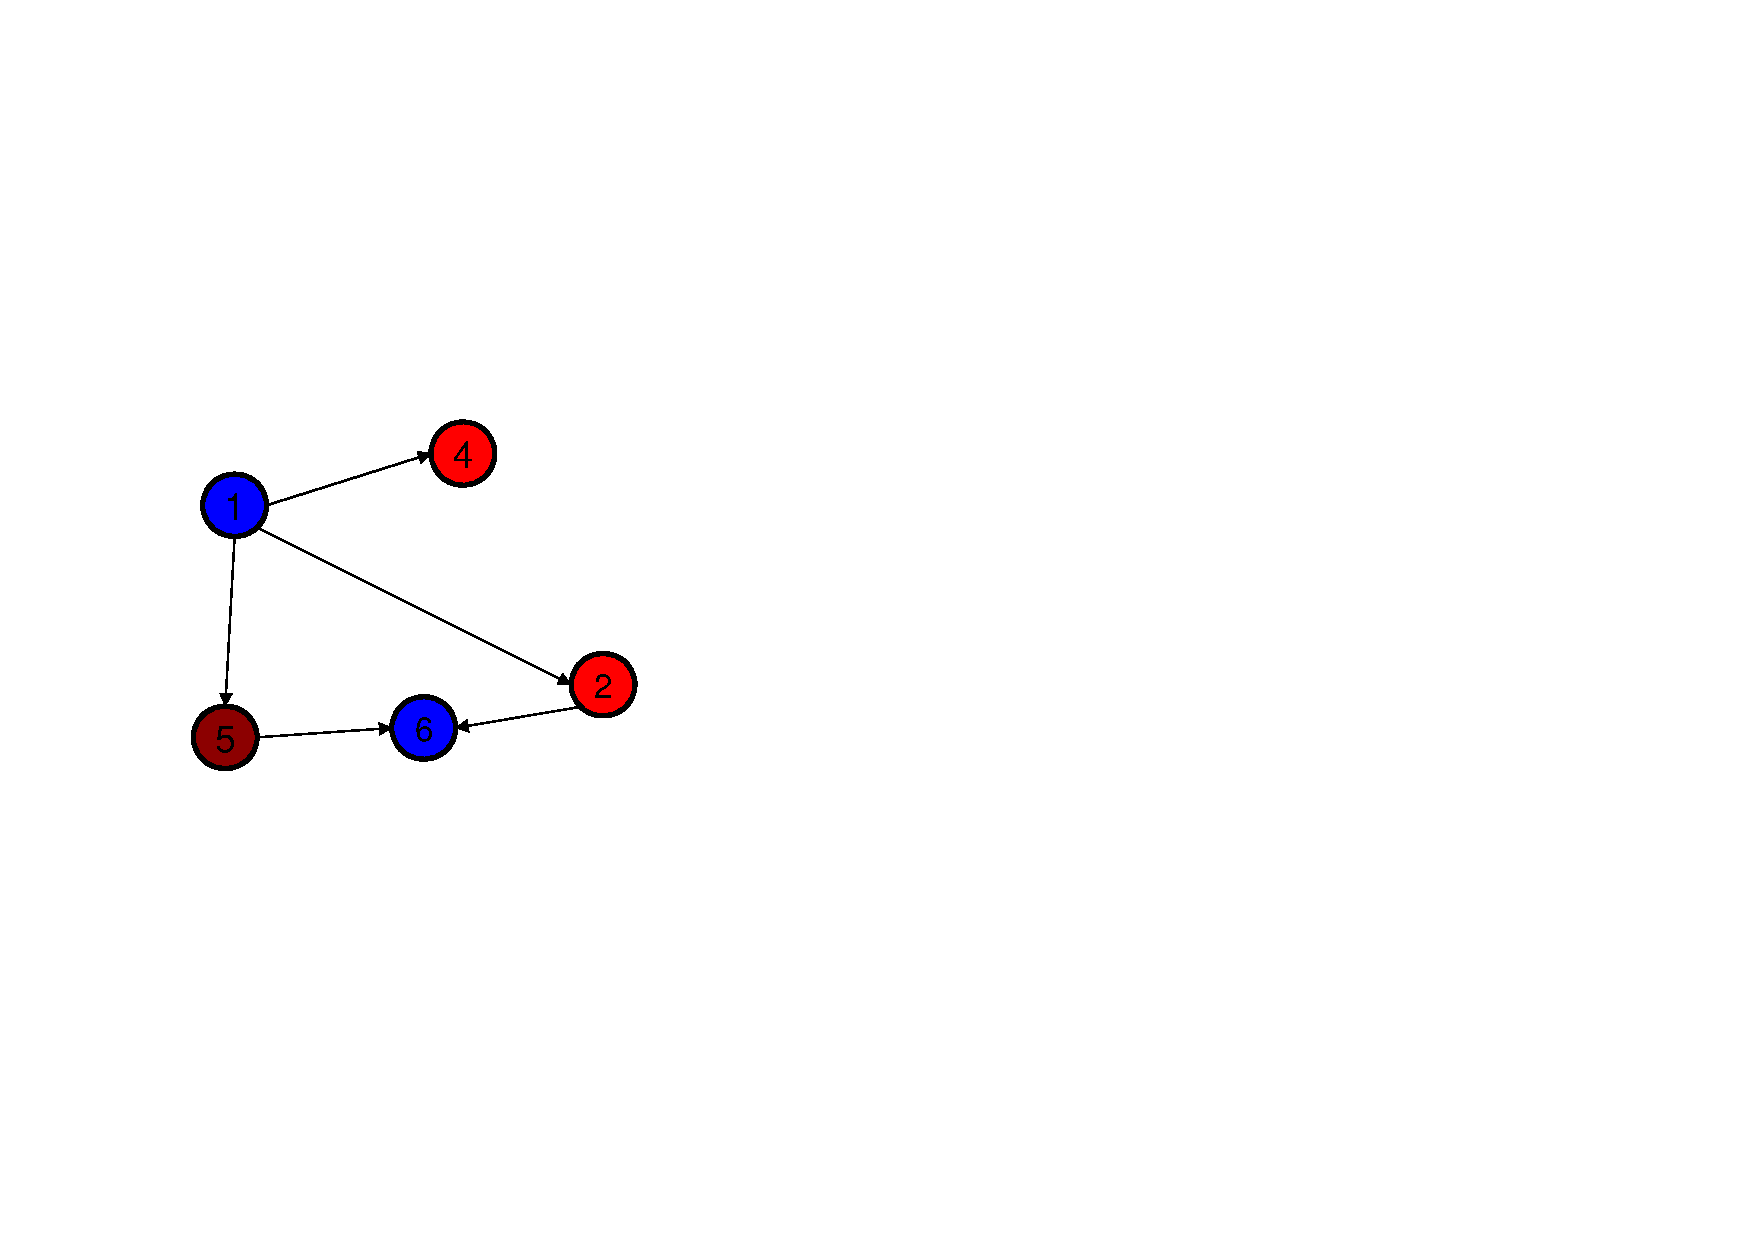
\includegraphics[scale=0.4]{figure/color_a.pdf}
}%
\caption{Coloring scheme for cyclical graph and acyclic graph.}
\label{fig:color_scheme}%
\end{figure}

Dynamic conflict list, which is an array used to store the vertices (or edges) to be processed in the subsequent iterations/loops, is widely used in both vertex-based and edge-based graph processing models. In graph coloring, the dynamic conflict list is used not only 
to maintain the upcoming workload, but also to store the candidate colors in the color array. 
A typical coloring algorithm traverses the color array to select a suitable color 
for current vertex. Because of the SIMD execution model in GPU, a massive number of threads access the 
color array simultaneously. The \emph{atomic} operation is widely 
used to manage the simultaneous accesses to a common array on GPU. Atomic operations suffer from the heavy overhead when there are frequent accesses. Moreover, atomic operations might result in a scattered conflict list,  
where the consecutive vertices are store far apart in locations.

Eliminating atomic operations on GPUs for maintaining 
the coloring array have been considered in previous work 
\cite{vldbcolor,Manycore}. Reference \cite{Manycore} 
is a representative graph coloring work on many-core architectures 
(including Xeon Phi and GPU). In their work, the authors defined two 
arrays. One is used to hold the forbidden colors for the active 
vertex $v$ while the other is used to select the smallest available 
colors. The two arrays are named \emph{VFORBIDDEN} and \emph{ASSIGNCOLORS}, respectively. 
The authors use atomic operations to maintain these two arrays. 
This approach is inefficient, because it cannot avoid the atomic 
operations fully and more memory space is needed for \emph{VFORBIDDEN} than 
traditional traversal algorithms. Figure \ref{fig:atomic} shows 
an example of typical color array on GPU with atomic operation. 
As we shown in figure \ref{fig:atomic}, when the algorithm colors 
vertex 1 and 5, the two threads that are processing these two vertices 
need to visit the color array simultaneously. To ensure that
both threads can get the right color, the atomic operation is needed. 

\begin{figure}[h]
\centering
\subfloat[Sample graph]{%
\label{fig:sample-graph}
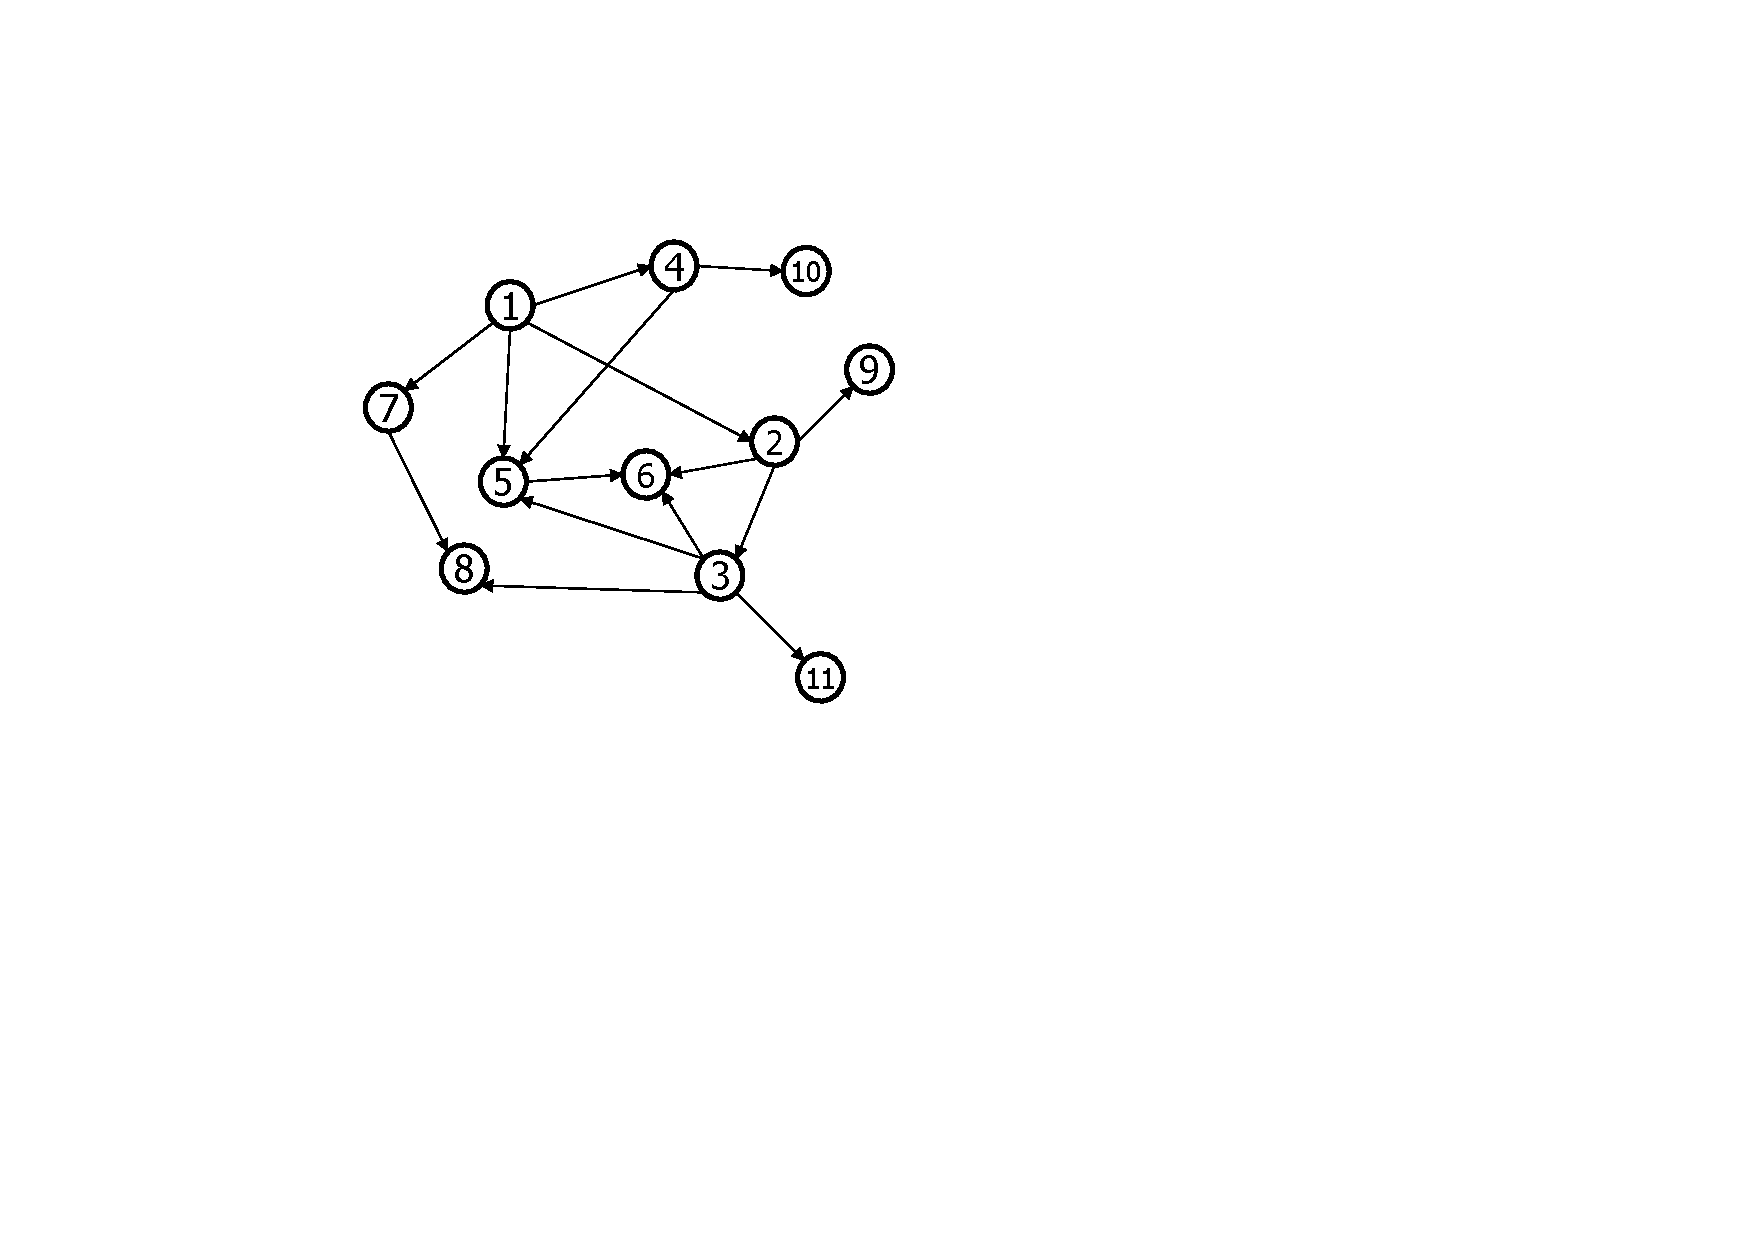
\includegraphics[scale=0.35]{figure/samplegraph_re.pdf}
}%
\subfloat[Color selecting]{
\label{fig:out-degree}
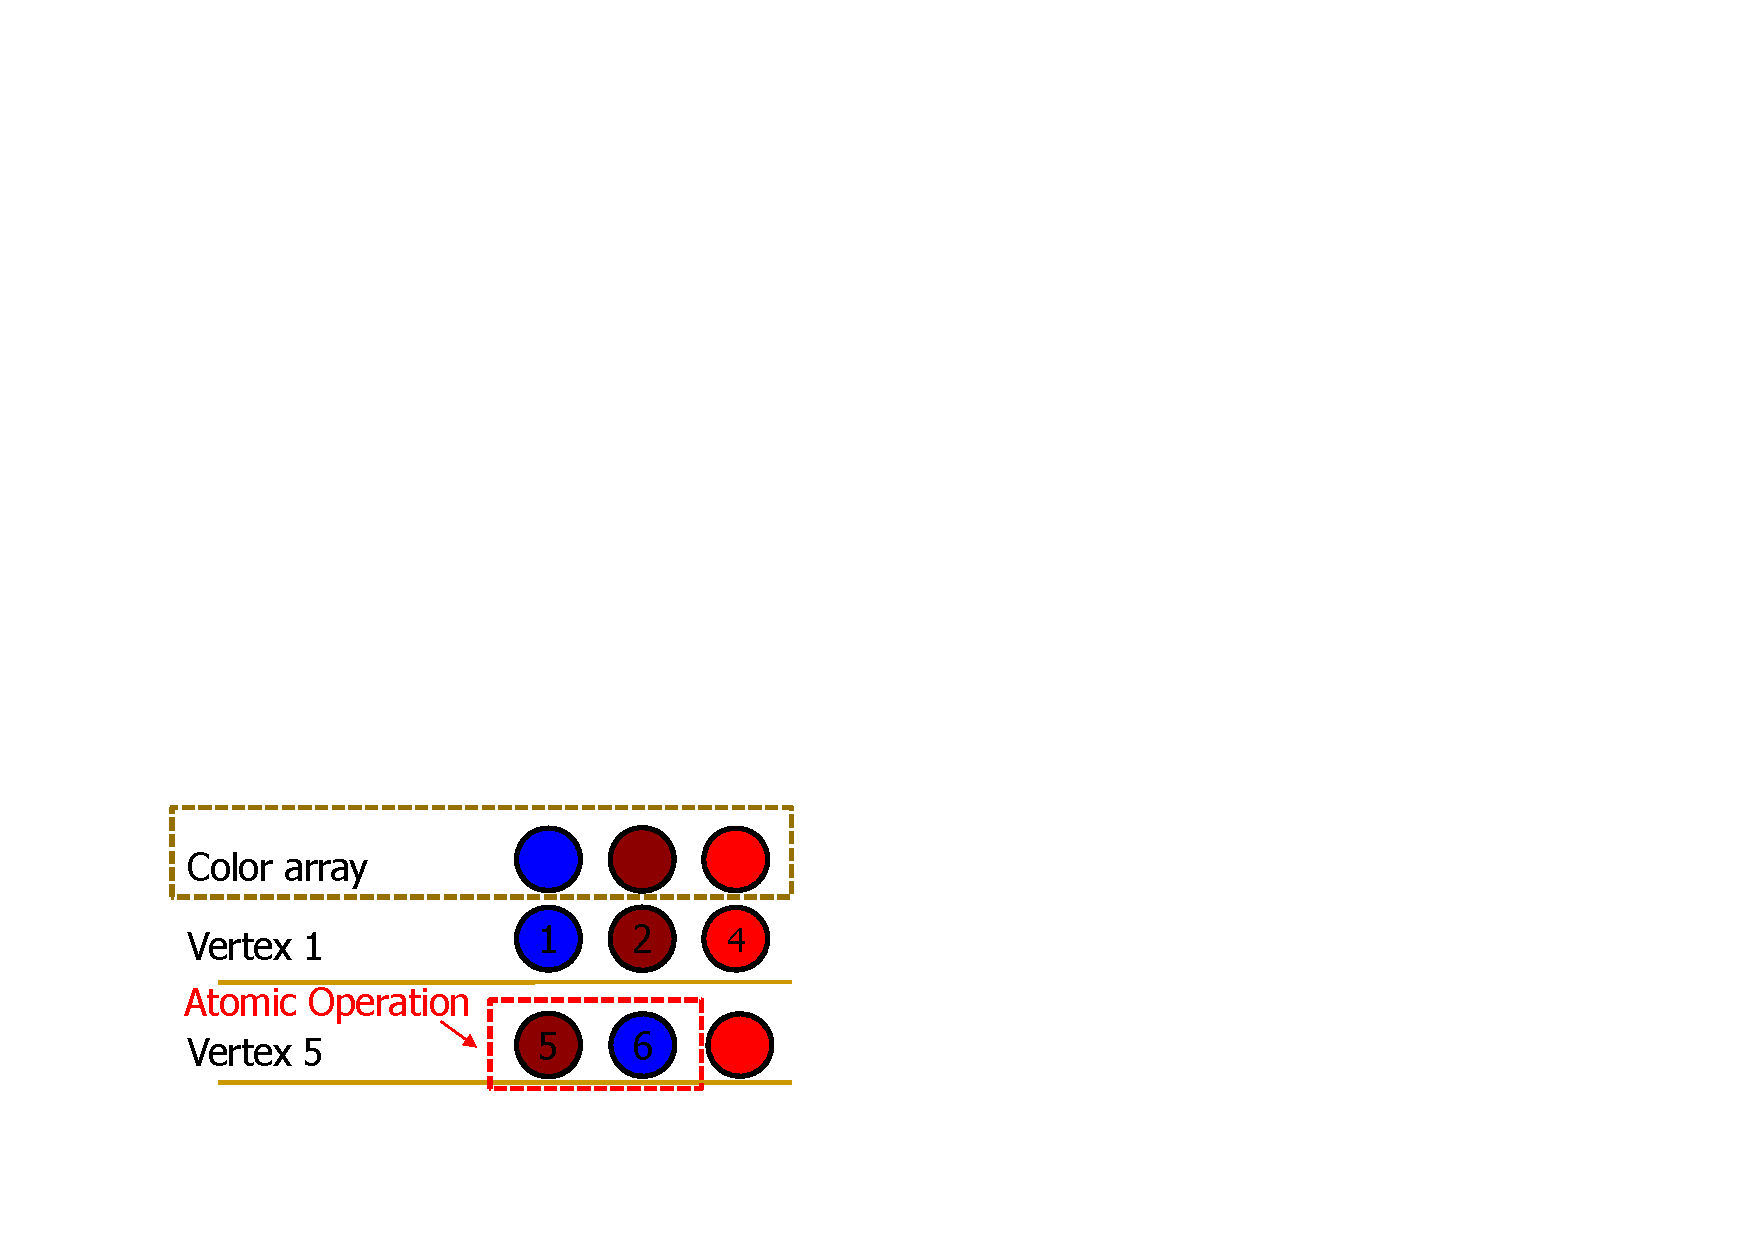
\includegraphics[scale=0.45]{figure/color-selecting.pdf}
}%
\caption{An example of typical color array with atomic operation.}
\label{fig:atomic}%
\end{figure}
 
There are several ways to resolve the color conflicting, such as selecting another new color randomly or assigning first available color when conflicts occur.  
But these methods may lead to a huge color set in the final result. Choosing the first available color is the most widely used method. In this method, 
the algorithm searches along the color array to find the first available color (i.e., the color is 
not used for previous vertices). As a massive number of threads are running in parallel for 
a GPU kernel, the atomic operation or lock is needed to ensure that every thread can 
find the right color. This will slow down the coloring process greatly. In Feluca, 
a top-down color selection scheme is 
proposed to select the suitable color for the conflicting vertices. This scheme can avoid the atomic operations fully. We detail the working of our color selection scheme next. 

As presented earlier in this section, we have transformed the graph to a directed acyclic graph (DAG). Our top-down coloring scheme starts coloring from the top level  (root) of the graph, and traverses the graph in the same way as the BFS (Bread-First-Search) algorithm. There are often multiple vertices in a graph level, which are colored by multiple threads in parallel. After a level of vertices are colored, the coloring scheme moves onto the next level in the DAG graph (hence a top-down coloring scheme), and the computation moves into next iteration. The process repeats until all vertices have been colored. 

A color array is used to hold all used colors. When a new color has to be used for a vertex, the new color is appended at the end of the color array. 

After a thread has colored a vertex in a level, it finds the neighbours of this vertex following its outgoing edge. The neighbours are the vertices in the next level, which are also the vertices ready to be colored in next iteration. When a thread is trying to color a vertex in an iteration (suppose in iteration $i$), it checks the colors assigned to this vertex's parents in last iteration (iteration $i-1$) and then assigns to this vertex the color that is immediately after the last color among all parents' colors in the color array. 

An example is illustrated in figure \ref{fig:colorsec} to show how our top-down coloring scheme works. The exemplar graph is still the one in figure 3. In figure \ref{fig:colorsec}, suppose the graph coloring is currently in iteration $i$. It can be seen from figure 3 that vertices 1 and 4 are the parents of vertex 5. Therefore when the coloring scheme colored vertices 1 and 4 in iteration $i-1$ (assume the colors assigned to vertices 1 and 4 are blue and red, respectively as shown in figure \ref{fig:colorsec}), it followed the edges $<1, 5>$ and $<4, 5>$ to find that vertex 5 is a vertex to be colored in iteration $i$. Now suppose the coloring scheme is trying to color  vertex 5 in iteration $i$. Our coloring scheme realizes that vertices 1 and 4 are the parents of 5. Then, it assign the color that is immediately after the colors of vertices 1 and 4 (blue and red), which is cyan, to vertex 5. The traditional coloring scheme would search the whole color array to find the first available color, which would assign ``dark red" to vertex 5 in this example. Our coloring scheme only needs to check the colors of the parents assigned in last iteration and does not need to search the entire color array. 

Our color chosen scheme only focuses on the current vertex and its parent vertices colored in last iteration. This design enables the GPU threads to update the colors of their current vertices in parallel without atomic operation/lock. 

\begin{figure}[h]
	\centering
		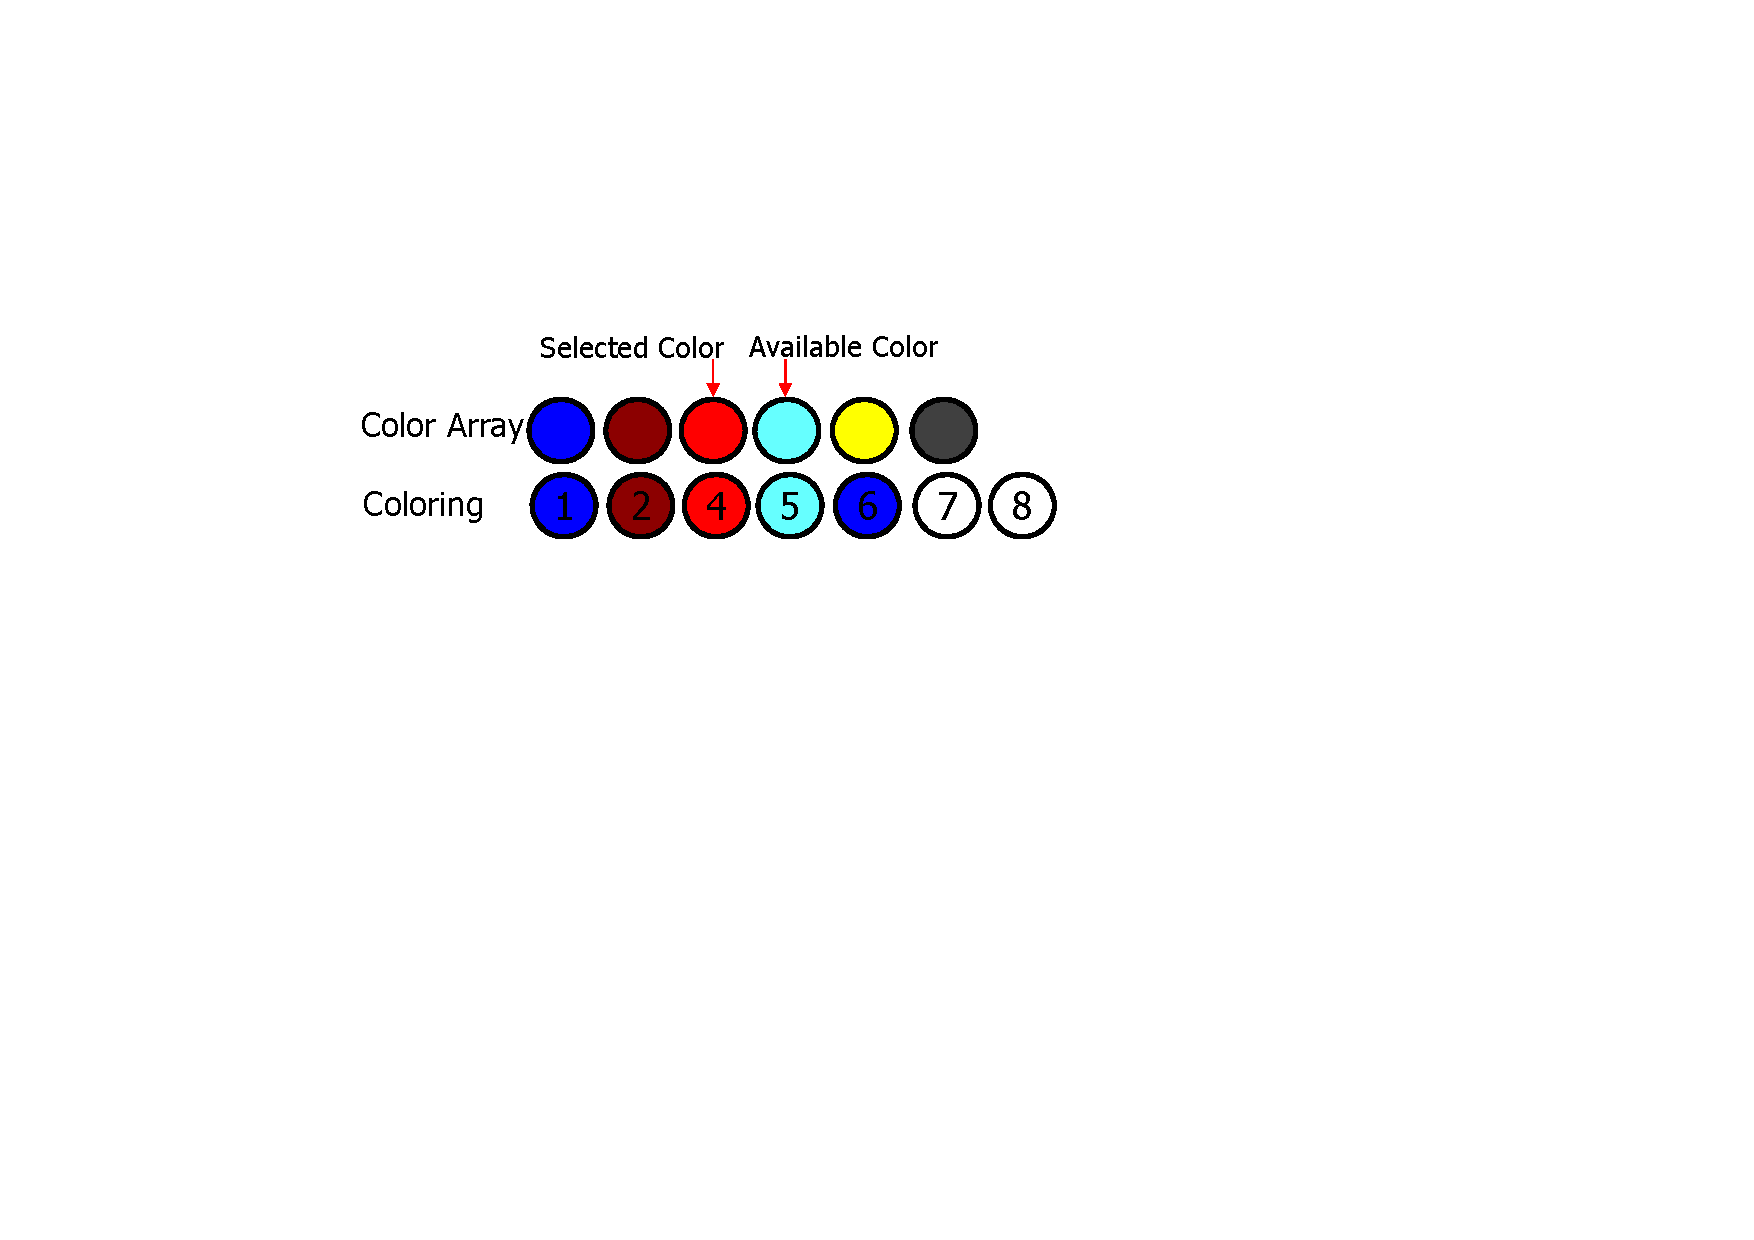
\includegraphics[scale=0.4]{figure/colorsec_re.pdf}
	\caption{The top-down coloring scheme in Feluca. The ``Selected color'' is the last color assigned to the parents of vertex 5 in iteration $i-1$. Then the color labelled as ``Available Color" will be assigned to vertex 5 in iteration $i$.}
	\label{fig:colorsec}%
\end{figure}

\subsection{Color-centric Coloring Paradigm}
\label{color-centric}

When GPU is used to accelerate graph processing, threads in GPU are organized in a grid and all the threads in a grid execute the same kernel function. The threads running a kernel are organized in a two-level hierarchy: a grid consists of a number of thread blocks and each block comprises a set of threads. It is a great challenge to parallelize the sequential spread coloring, because coloring the vertices in iteration $i$ depends on the results of iteration $(i-1)$.
In order to improve the degree of parallelism of the sequential spread stage in Feluca, we proposed a new coloring scheme, called the color-centric scheme. 
The traditional algorithm for sequential spread coloring is vertex-centric, i.e., finding a suitable color for each vertex. In our color-centric scheme, we find all suitable vertices for each color, which is presented in detail next. 

After the first coloring stage (the recursion stage) is finished, we record all the remaining vertices which have not converged to the final colors yet (called uncolored vertices).  
In the color-centric scheme, for each color, we generate a thread block to find in the list of remaining un-colored vertices all vertices that can be assigned with this color. A thread block starts with the uncolored vertices in the first graph level, and moves down the graph levels until all uncolored vertices have been colored. 

In the color-centric scheme, different thread blocks find vertices for different colors in parallel. We develop two parallelization strategies to run the thread blocks for each color. In the first parallelization strategy, we set the number of colors needed for the remaining uncolored vertices. We then generate a thread block to find all vertices for each color. In particular, a thread block for a color collectively find all vertices that do not have direct links between any two of them and assign all these vertices to this color. We start the execution of all thread blocks at the same time. In this strategy, it is possible that different thread blocks assign different colors to the same vertex. When this happens, the vertex keeps the color which has the smallest color ID among the conflicting colors. The shortcoming of this parallelization strategy is that we have to first set the number of colors for the remaining uncolored vertices. We cannot accurately know the exact number of colors needed. On one hand, if the number of colors is set too low, it is impossible to deliver the final coloring plan which does not contain conflicting. On the other hand, if the number is set too high, the number of colors in the final coloring plan will be much higher than that in the optimal coloring plan. 

In the second parallelization strategy, we do not start all thread blocks at the same time, but run the thread blocks in pipeline. In particular, we first start the thread block for the first color. The thread block starts with find all uncolored vertices in the first level of the graph that can be assigned to the first color. After the first level is processed, the thread block moves to the second level and repeats the process. While the thread block for the first color is processing the second level, we start the thread block for the second color and start to find all remaining uncolored vertices that can be assigned to the second color. Similarly, when the thread block for the first color moves to the third level, the thread block for the second color moves to the second level and the thread block for the third color start processing the first level. The pipeline goes on until all uncolored vertices after the recursion stage have been colored. In the second strategy, we do not have the problem that we may set the number of colors too high. When all vertices have been colored, the pipeline stops and the number of used colors then is the number of colors in the final coloring plan. Our experiments show that the first and second parallelization strategies have similar running performance. But the second strategy typically uses a fewer number of colors than the first strategy. Therefore, we use the second parallelization strategy in the sequential spread stage in Feluca. 

\subsection{The Edgelist Graph Representation}
\label{edgelist}
A GPU can reach its peak memory 
access bandwidth only when the algorithm has a regular memory access pattern, 
i.e., the data accessed by the consecutive threads of a warp occupies the 
contiguous memory locations. 
When there is no a regular memory access pattern, a naive solution to improve the GPU memory access efficiency is to sort 
the edges by source vertex ID, which is shown in figure \ref{fig:edgelistrep}. 
Figure \ref{fig:edgelistrep} shows the edgelist representation of the graph in figure \ref{fig:sample-graph}. 
The graph has 11 vertices and 15 edges. The 15 edges are partitioned into 4 edge blocks. In this partition, the edges are 
sorted in the order of their source vertex IDs and every edge block contains 4 edges. Suppose that 
a warp contains 4 threads. Then a warp can process the whole block.
But in this partition, the edges with source vertex ID 3 are allocated to 2 
blocks. Hence, the threads processing the edges with source vertex 2 in 
block 2 need to wait for the threads which process the edges with source 
vertex ID 3. It is also the case for the threads which process 
with source vertex 4. When processing the real-world graphs, the edges of 
high degree vertices may be scattered in several blocks. On the other hand, a block 
may contain the edges from more than one low-degree vertex. Under this circumstance the computing load of different edge blocks vary, which will cause 
the threads in a thread block to wait for other thread blocks with more computing load. 

\begin{figure}[h]
\centering
\subfloat[The edgelist representation of the graph in figure \ref{fig:sample-graph}.]{%
\label{fig:edgelistrep}
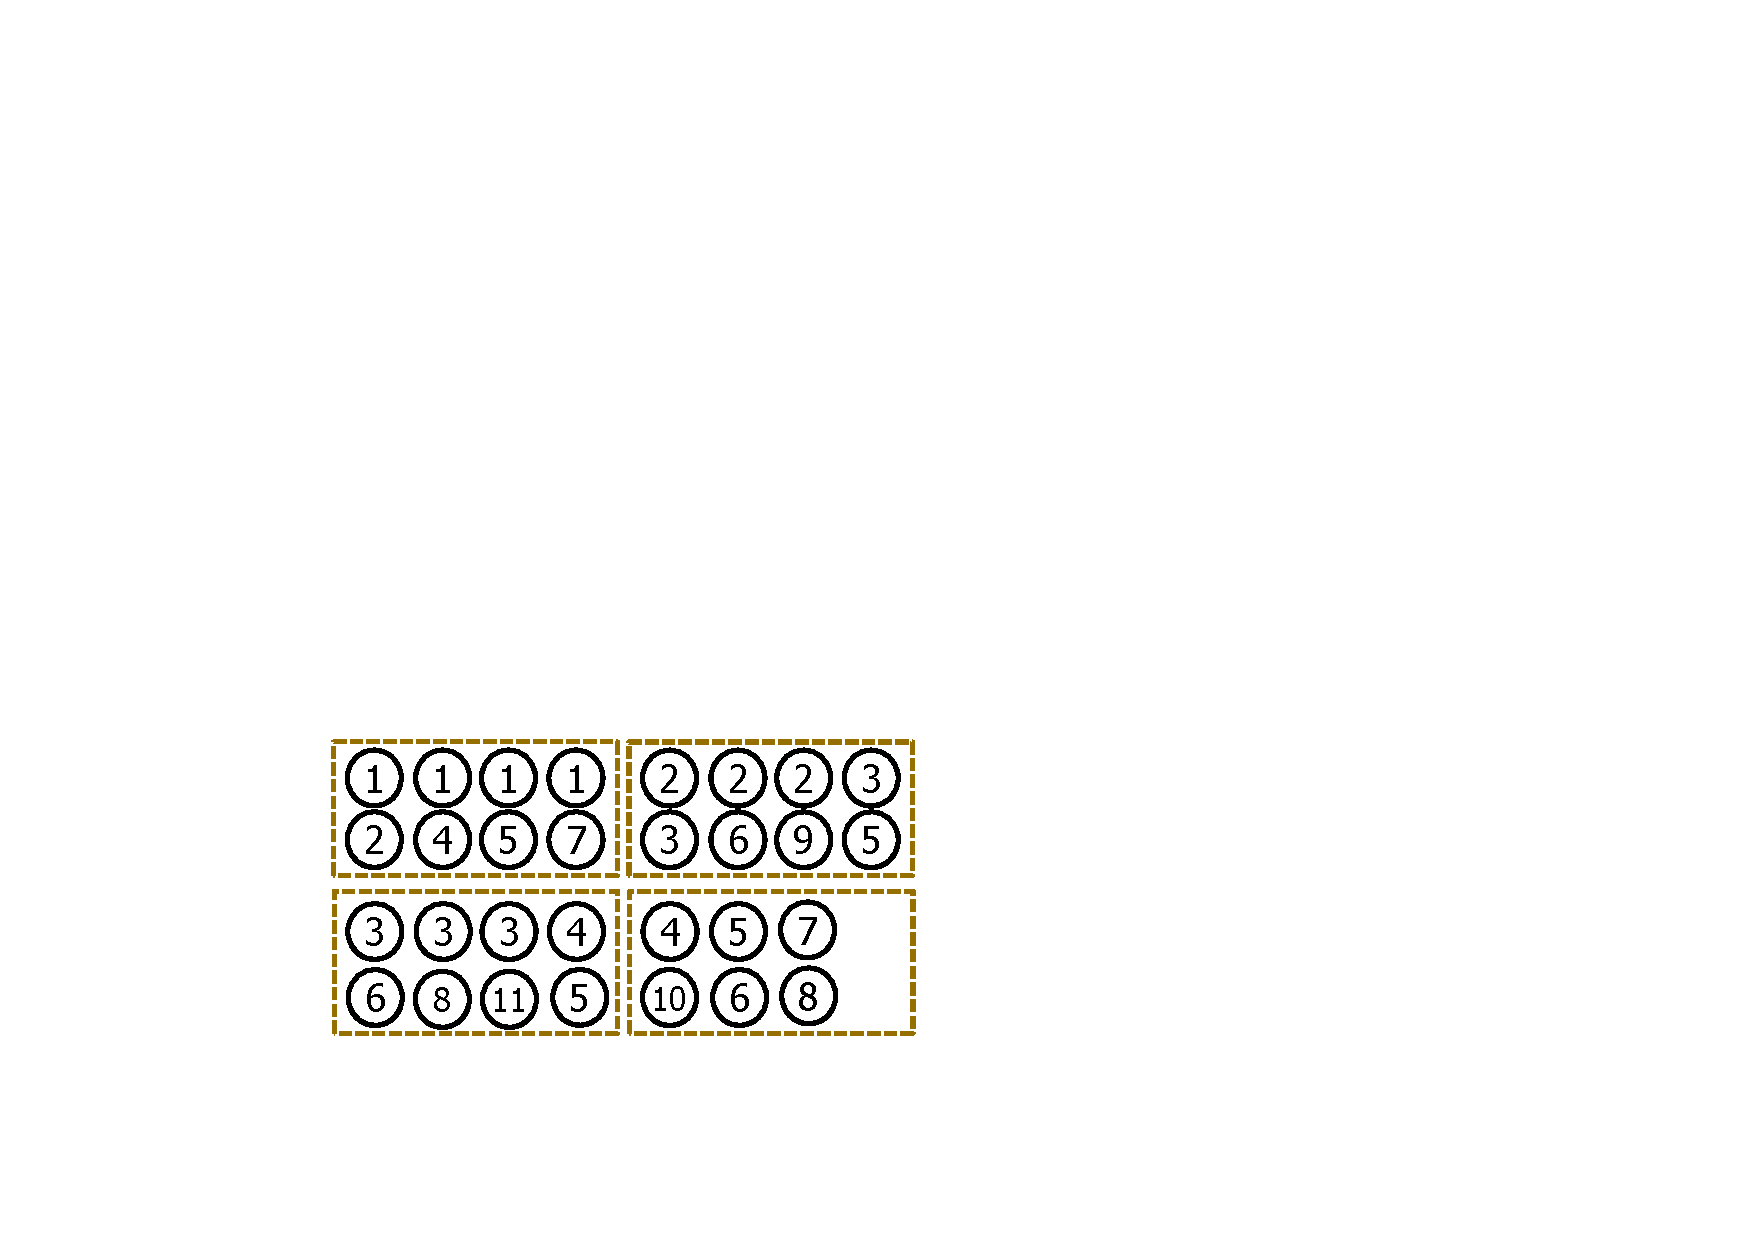
\includegraphics[scale=0.4]{figure/edgelist_re.pdf}
}%
\subfloat[The ordered graph with virtual edges.]{
\label{fig:rep}
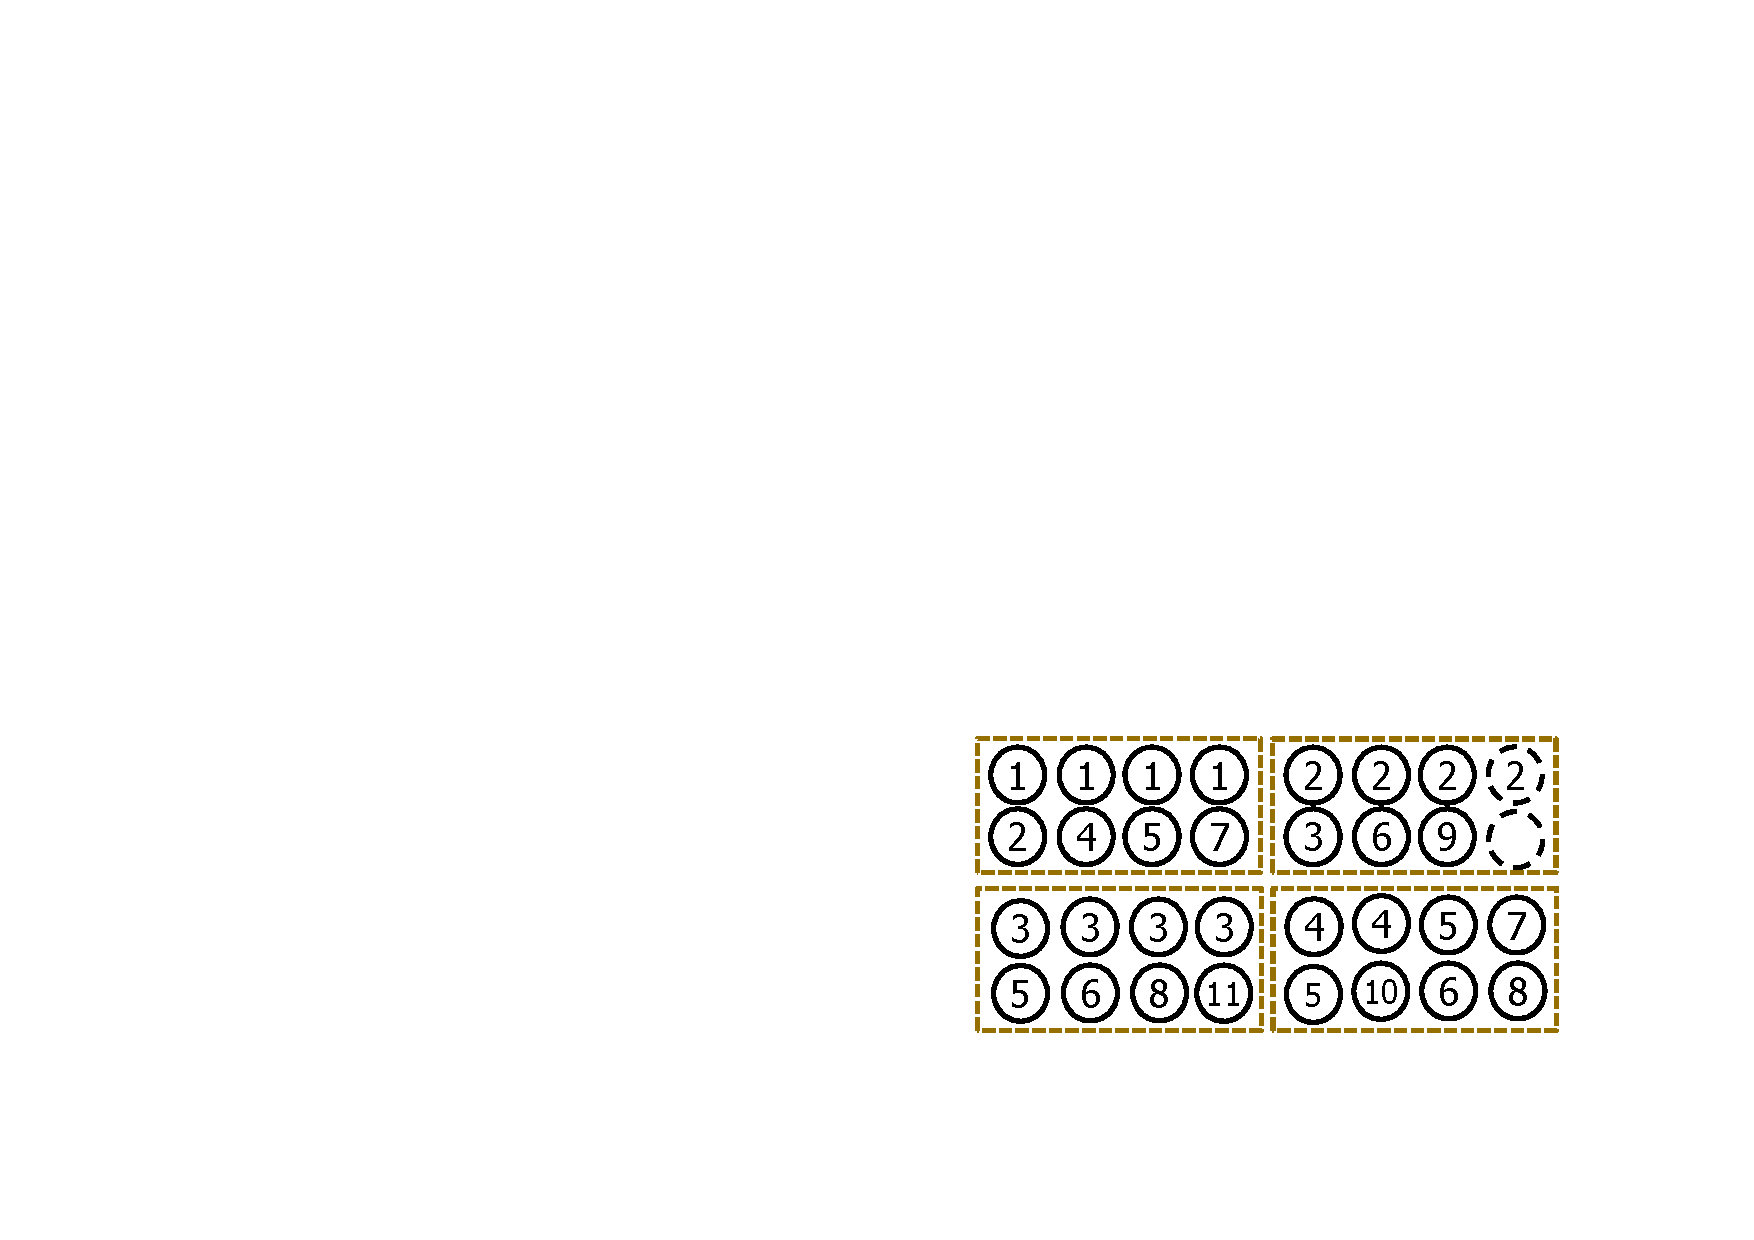
\includegraphics[scale=0.4]{figure/rep_re.pdf}
}%
\caption{An example of ordering the graphs by adding virtual edges.}
\label{fig:virtual_edges}%
\end{figure}

In order to address this problem, Feluca adds some virtual edges, which do 
not take any memory space, in the edgelist-based graph representation such that either the edges in an edge block have the same source ID or an edge block contains all edges from different vertices. 

For example, We add a virtual edge with source vertex ID 2 as shown in figure \ref{fig:rep}. In the ordered graph, all the 
edges with source vertex ID 1, 2 and 3 are located in a single warp and all the 
remaining edges are located in the same warp (i.e., the warp contains all edges for vertice 4, 5 and 7). This representation can avoid the 
overhead that the threads wait between the edges with source vertex 2 and 3. As edges 
are sorted in the order of the source vertex ID in the grid, continuous and coalesced memory 
access pattern can be achieved.